%1521001##1##.tex
\documentclass[12pt,letterpaper]{article}
\usepackage{mathptmx}
\usepackage[margin=1in]{geometry}

\usepackage{setspace}
\doublespacing
  
\usepackage{amssymb,latexsym}
\usepackage[round,sort]{natbib}
\usepackage{fancyhdr}
\usepackage{lastpage}
\usepackage{graphicx}
\graphicspath{ {qe1/} }

% Bold Table and Figure captions
\usepackage{caption}
\captionsetup{figurename=FIGURE}
\captionsetup{tablename=TABLE}
\captionsetup[figure]{labelfont=bf}
\captionsetup[table]{labelfont=bf}
  
% Turns off all section numbering
\setcounter{secnumdepth}{0} 

  % Places all tables at end of document and creates AOM-style table-here placeholders
  \usepackage[nolists]{endfloat} % Places all figures and charts at end of manuscript and adds 'insert table x about here' lines.
  \renewcommand{\figureplace}{
    \begin{center}
    \begin{singlespace}
    ------------------------------------\\
    Insert \figurename \ \thepostfig\ about here.\\
    ------------------------------------
    \end{singlespace}
    \end{center}}
  \renewcommand{\tableplace}{%
    \begin{center}
    \begin{singlespace}
    ------------------------------------\\
    Insert \tablename \ \theposttbl\ about here.\\
    ------------------------------------
    \end{singlespace}
    \end{center}}

  \usepackage{titlesec}
   \titleformat{\title}
       {\filcenter\normalfont\bfseries\uppercase}{\thetitle}{1em}{}
  \titleformat{\section}
    {\filcenter\normalfont\bfseries\uppercase}{\thesection}{1em}{}
  \titleformat{\subsection}
    {\normalfont\bfseries}{\thesubsection}{1em}{}
  \titleformat{\subsubsection}[runin]
   {\normalfont\bfseries\slshape}{\thesubsubsection}{1em}{\hspace*{\parindent}}
       
\usepackage{tabu}
\usepackage{textcomp}
\usepackage{listings}
\usepackage{hyperref}
\usepackage{verbatim}
\usepackage{tabu}
\hypersetup{
    colorlinks=true,
    linkcolor=blue,
    filecolor=cyan,      
    urlcolor=cyan,
    citecolor=blue,
}
\lstset{
basicstyle=\ttfamily,
columns=flexible,
breaklines=true
}
\newenvironment{hypothesis}{
  	\itshape
  	\leftskip=\parindent \rightskip=\parindent
  	\noindent\ignorespaces}

\fancypagestyle{plain}{
  \renewcommand{\headrulewidth}{0pt}
  \fancyhf{}
}	


\begin{document}
\title{Embedded Agency in Institutional Fields: Developing Theory from a Matching Game}
\date{}
\maketitle

\begin{abstract} 
\normalsize 
We apply a formal model to understand the effects of the relative learning rates of embedded agents and the institutional field on organizational outcomes. Applying the principle of reinforcement learning in a repeated game of matching, we generate hypotheses for specific configurations of agents and fields. We contribute to the theory on embedded agency in institutional fields with a nuanced and dynamic view of the role of the relative rates of learning in achieving matching outcomes in organizations.
\end{abstract}


{\textbf{Keywords:} \\\indent Embedded Agency, Agent Based Modeling, Reinforcement Learning}

\newpage
\pagestyle{fancy}
\fancyhf{}
\lhead{Embedded agency in institutional fields}
\rhead{\thepage}
%\section{Introduction}\label{S:Introduction}
\begin{center}
\textbf{Embedded Agency in Institutional Fields: Developing Theory from a Matching Game}
\end{center}
Our understanding of  institutional phenomena has come a long way since \cite{Selznick1957} made the observation that organizations adopted new goals suited to existing structures  instead of changing the structures that may have outlived their utility. 

The rest of this article is organized as follows. In the following section, we summarize the key constructs and definitions in institutional theory that we build upon in this article. We then present the assumptions and the formal definitions for the model. A subset of our initial results from the computer simulations of the model are then presented in the following section. We propose hypotheses on the dynamics of embedded agency and their institutional fields based on our findings from our computer simulation. We conclude with a call for continuing this path for theory development, and for empirical studies to use the theoretical frames developed here for both conceptual synthesis and empirical validity of the hypotheses proposed. The Python code used for this modeling work is provided in the appendix section.

\section{Background}
Prior to describing our formal model, we discuss here some of the salient constructs within institutional theory that provide both the motivation as well as the vocabulary appropriate to our discussion. \cite{Scott1995} visualized institutional fields as a community of organizations that partakes of a common meaning system and whose participants interact more frequently and fatefully with one another than with actors outside the field. This definition is similar to that of \cite{Dimaggio1983} who defined institutional fields as those organizations that in the aggregate constitute a recognized area of institutional life: key suppliers, resource and product consumers, regulatory agencies, and other organizations that produce similar services or products. 

\section{Model}

We develop a simple model consisting of two players who participate in a repeated game of matching \footnote{I am grateful to Phanish Puranam for having introduced me to this model of reinforcement learning during a workshop at the Indian Institute of Science on 16th December, 2016. His definitions and code have been extensively reused in this work.}. Our study will assume the two players to be the institutional field (F), and the embedded agent (A). In each time period each of the players can make one of two decision choices 0 or 1. At the start of the game, the institutional field F choses choice 0 with probability $p_{0,F}^0$ and choice 1 with probability $1 - p_{0,F}^0$. Similarly, at the start of the game, the embedded agent A choses choice 0 with probability $p_{0,A}^0$ and choice 1 with probability $1 - p_{0,A}^0$. When the choices of the institutional field F and embedded agent A match in a time period, they each get a payoff of 1 in that period. Otherwise they each get a payoff of 0. The payoffs are captured by the matrix in Table ~\ref{payoffmatrix}

\begin{table}
\begin{centering}
\caption {Payoff Matrix}
\label{payoffmatrix}
{\tabulinesep=1.4mm
\begin{tabu}{|c|c|c|}
\hline
&$choice_F(t) = 0$&$choice_F(t) = 1$\\\hline
$choice_A(t) = 0$&$[payoff_F(t),payoff_A(t)]=[1,1]$&$[payoff_F(t),payoff_A(t)]=[0,0]$\\\hline
$choice_A(t) = 1$&$[payoff_F(t),payoff_A(t)]=[0,0]$&$[payoff_F(t),payoff_A(t)]=[1,1]$\\\hline
\end{tabu}}

\end{centering}
\end{table} 

To help improve the intuition in the analysis, we define a few categories. For the learning rate $\phi$, we define three categories: Slow ($\phi <= 0.05$), Medium ($0.05 < \phi <= 0.3$) and Fast  ($0.3 < \phi <= 0.7$). In the models to follow, we additionally assume that agents may have learning rates of Slow, Medium and Fast, while Fields may have learning rates of Slow and Medium. The determination is made building on the assumption that the institutional field may learn at a rate no faster than that of any of its constituent embedded agents. $choice(t)$ is either 0 or 1 for each player, with 0 being picked with a probability of $p_{t,F}^0$ by the field F and 0 being picked with a probability of $p_{t,A}^0$ by the agent A. We now define the following categories to assist in referring to prior probabilities of player choice. 

\subsection{Field Start Position}
The Field Start Position is a characterization of the choice preference of the institutional field at the start of the interaction. The institutional field may chose an outcome 0 with probability  $p_{0,F}^0$. We visualize the institutional field\textquotesingle s initial preference as being Left (L) when $p_{0,F}^0$ takes a value between zero and 0.1, as Left of Center (LC) when $p_{0,F}^0$ takes a value between 0.1 and 0.35, as Center (C) when $p_{0,F}^0$ takes a value between 0.35 and 0.65,  as  Right of Center (RC) when $p_{0,F}^0$ takes a value between 0.65 and 0.9, and as Right (R) when $p_{0,F}^0$ takes a value between 0.9 and 1. For the analysis in this article however, we restrict ourselves to only two of the five Field Start Positions, viz: Right of Center (RC) and Right (R). 
\subsubsection{The third level section}
We do so since the scale is symmetric across the Center (C), any initial mapping of Left (L) and Left of Center (LC) can be mapped onto an equivalent Right (R) or Right of Center (RC) configuration. The Center (C) configuration may be an interesting one to consider, but has had to be dropped here to stay focussed on environments where the institutional fields have a clear directional preference to start with.


\begin{figure}[h]
\begin{centering}
  \caption{}
  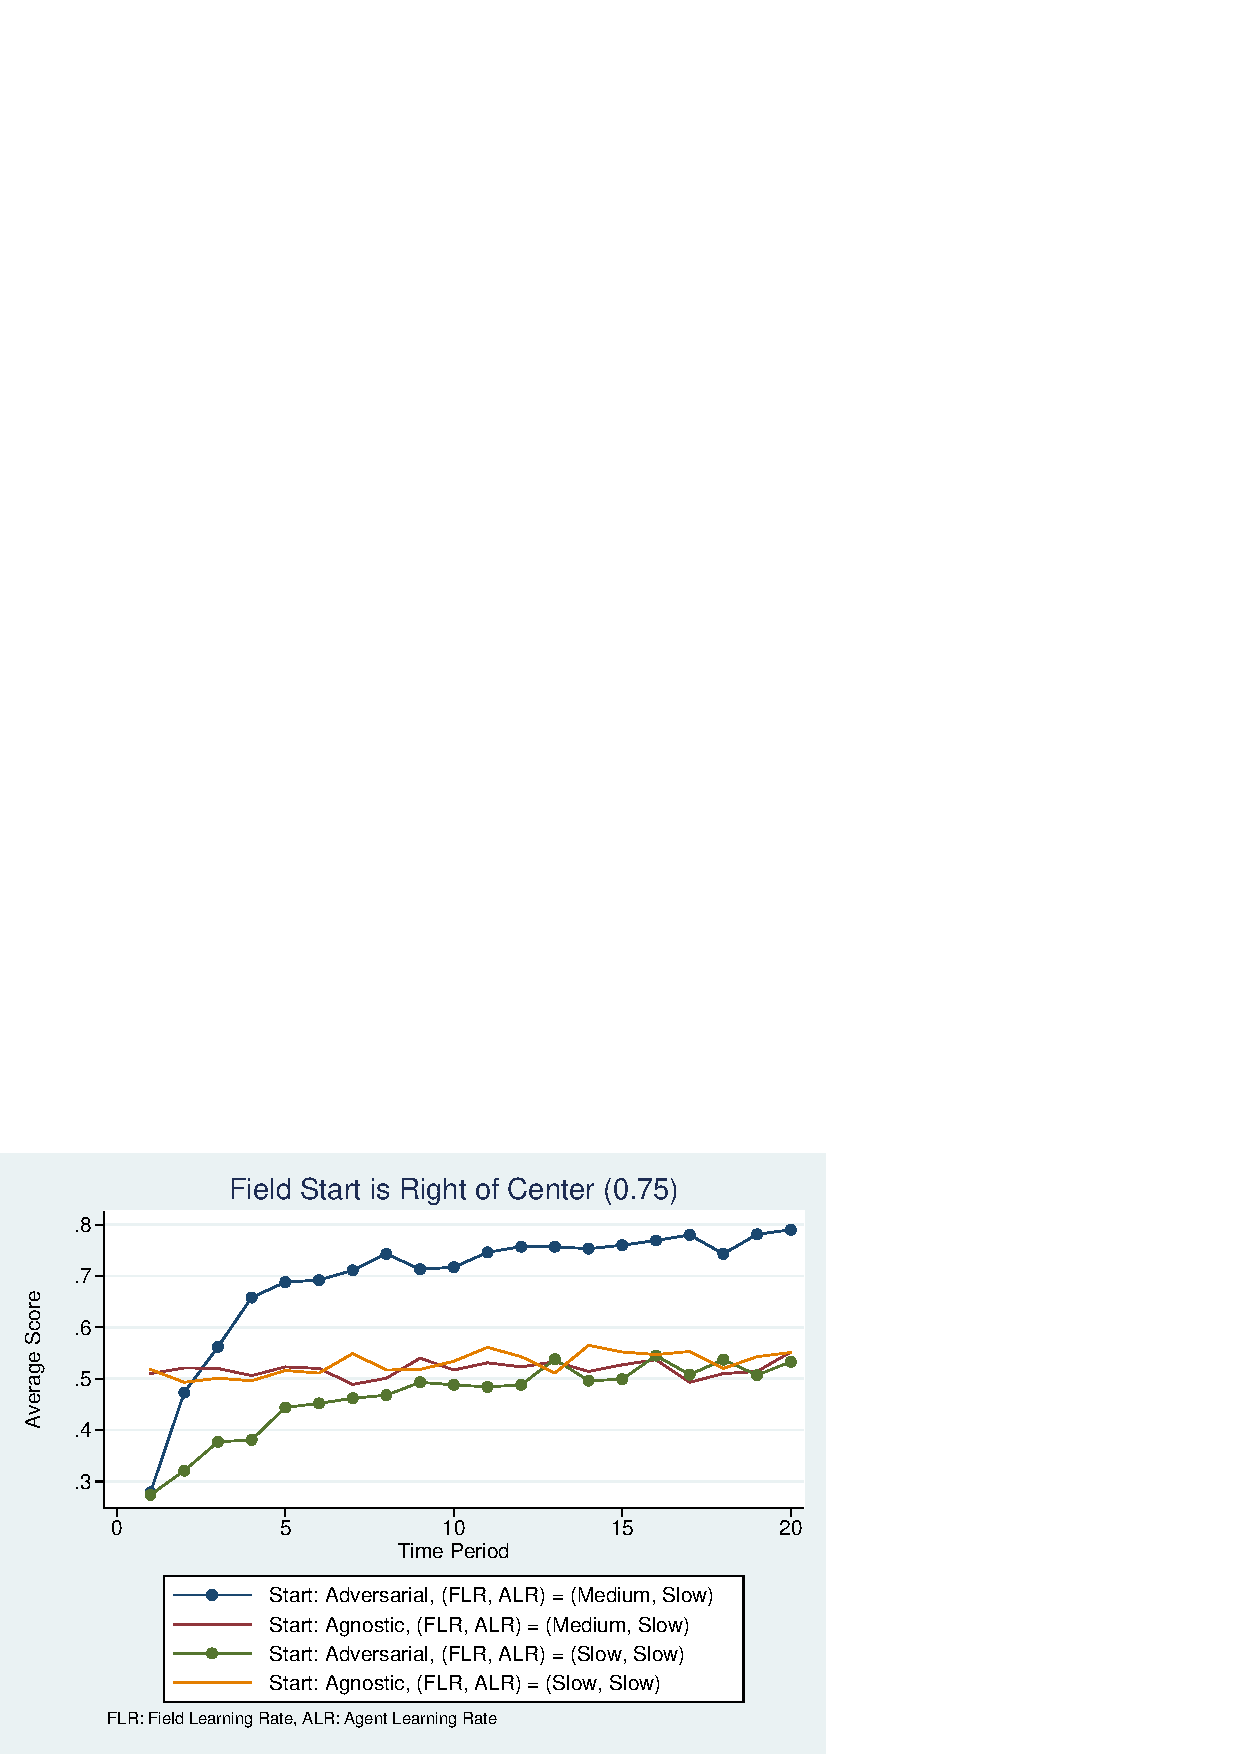
\includegraphics[width=\textwidth]{frcmedium3a}
  \label{fig:3a}
\end{centering}
\end{figure}

\section{Discussion}
Having laid out the formal model and having described the assumptions and classifications made in the previous section, we now consider if the model described above is a reasonable abstraction of the phenomenon that we wish to theorize upon. We consider this in the current section.

\section{Interpretation of Model Results}
In order to understand the effect of each change on the outcome, we proceed to understand the effects of field configuration and agent configuration on overall outcome one change at a time. Figure ~\ref{fig:3a} lays out the average score charts for four agent-field combinations while enforcing the field to start in Right of Center (this is the same as saying $p_{0,F}^0 = 0.75$). Figure ~\ref{fig:3a} demonstrates that an adversarial agent with a slow rate of learning ($\phi_A = 0.05$) is likely to get stuck at a peak average performance of around 0.5, whereas one in medium learning rate field is likely to reach a peak average performance of close to 0.8 (This is the comparison of the two dotted lines graphs in blue and green). 

On the other hand, we notice that agnostic agents do similarly despite changes in the rate of learning of the field F. The interesting result from Figure ~\ref{fig:3a} is that though adversarial agents start off with contradictory preferences to the field, they end up with a higher average score than the agnostic agents who start off with a better alignment (0.5 is more aligned to 0.95 than is 0.05). The logic for this result is that the adversarial agent is actually adapted by the field F due to its relatively higher learning rate. In the case of the adversarial agent in the (Slow, Slow) configuration, the agent was stuck with $p_{t,A}^0$ closer to 0.5 with the field F unable to pull that agent A up quickly enough due to it's slow rate of learning. This (adversarial agent in a (Slow, Slow)) configuration is therefore a good candidate for a change in setting.

\begin{hypothesis}
{Hypothesis 1a: When the institutional field is open to influence, slow learning adversarial agents will raise overall performance higher than slow learning agents with a neutral orientation\\}
\end{hypothesis}

Indeed, Figure ~\ref{fig:3a} demonstrates that the agnostic agents who begin being neutral to either outcome are able to use their superior learning rates to achieve a higher level of overall performance. This trend is confirmed further in Figure ~\ref{fig:3a} where the learning rates of agents are increased even further to \textquotesingle Fast\textquotesingle .


\begin{hypothesis}
{Hypothesis 2a: For the same initial outcome preferences,  the overall performance score varies curvilinearly with difference in the rates of learning of the agent and the institutional field\\}
\end{hypothesis}

\section{Limitations and Future Work}
The formal computational modeling approach to theorizing organizational phenomena comes across as being both valuable and challenging simultaneously. While the fine grained control and possibility of step by step changes in experiments allows for a detailed understanding of micro phenomena, the very flexibility also creates a problem of plenty. However, with the appropriate priorities this should be a good problem to have.


\section{Conclusion}
We started out attempting to improve our understanding of the mechanisms behind the embedded agent - institutional field engagement. We captured the dynamics of the embedded agent - institutional field relationship as a function of their relative learning rates over repeated encounters in a game of matching. Despite focusing on a sub-set of potential states, we were able to demonstrate multiple situations where seemingly counter-intuitive priors lead to better outcomes. Our work here contributes to a nuanced and deeper understanding of the dynamics of the embedded agent - institutional field relationship, and a potential mechanism by  which changes in this setting may affect organizational outcomes.  \cite{Zhao2006}

\begin{comment}
\section{Acknowledgements}
I am heavily indebted to Abhoy Ojha for having set the bar for this paper high. I am indeed the biggest beneficiary of the expectation of as full a paper as possible. My ability to do this work was also contributed to by Sai Yayavaram, who introduced me in June 2015 to the wonderful world of computational modeling, and to Phanish Puranam who helped me with thinking about simple agent based models for modeling organizational phenomena. All mistakes made here are completely mine. 
\end{comment}

\newpage
\begin{singlespace}
\bibliography{/Users/anu/code/bibliography/aiyenggar} 
\bibliographystyle{ai-amjlike}
\end{singlespace}

\newpage
\appendix
\begin{singlespace}
\section{APPENDIX A: Simulation Code}
\lstinputlisting{qe1/matchingEmbeddedAgency.py}
\end{singlespace}

\end{document}
